\documentclass[12pt]{article}

\usepackage[a4paper, margin=1in]{geometry}
\usepackage{graphicx}
\usepackage{multicol}
\usepackage{titlesec}
\usepackage{authblk}
\usepackage{setspace}
\usepackage{fancyhdr}
\usepackage{abstract}
\usepackage{caption}
\usepackage{float}
\usepackage{parskip}
\usepackage[absolute,overlay]{textpos}
\usepackage{lipsum}



% Remove paragraph indent
\setlength{\parindent}{0pt}

% Title formatting
\titleformat{\section}{\large\bfseries}{\thesection}{1em}{}
\titleformat{\subsection}{\normalsize\bfseries}{\thesubsection}{1em}{}

% Header
\pagestyle{fancy}
\fancyhf{}
\renewcommand{\headrulewidth}{0pt}
\fancyfoot[C]{\thepage}

% Set units for absolute positioning
\setlength{\TPHorizModule}{1mm}
\setlength{\TPVertModule}{1mm}

% Title + Author
\title{
\vspace{-2em}
\rule{\textwidth}{0.4pt} \\[0.5em]
\textbf{\LARGE Benchmarks and Improvements on\\ Multi-Label Chest X-ray Classification\\ Using a Lightweight CNN Architecture} \\
\rule{\textwidth}{0.4pt}
}
\author{
Ahmad Hamadi\textsuperscript{1}, Jared Paul\textsuperscript{1}, Gurnoor Bal\textsuperscript{1}, Hamza Issa\textsuperscript{1}, Harrison Chiu\textsuperscript{1} \\
\textsuperscript{1}Department of Computing and Software, McMaster University, Hamilton, Ontario, Canada \\
\texttt{Email: hamada11@mcmaster.ca, paulj20@mcmaster.ca, balg3@mcmaster.ca, issah3@mcmaster.ca, chiuh6@mcmaster.ca}
}
\date{}

\begin{document}

% Place logo at top right
\begin{textblock}{40}(158,6)
    
\includegraphics[width=2.8cm]{McMaster_Faculty_of_Engineering_logo.png}
\end{textblock}

\maketitle

\vspace{-1em}
\noindent\textit{Capstone Research Paper}

\vspace{1em}

\begin{abstract}
\noindent
\textbf{Abstract—} Chest radiography is a foundational imaging tool in clinical diagnostics. In this work, we present a lightweight convolutional neural network for multi-label classification of chest X-rays. We explore different backbone architectures, loss functions, and data balancing strategies to optimize classification performance on the NIH ChestX-ray14 dataset. Our findings demonstrate that with careful tuning, compact models can achieve performance comparable to larger networks—while remaining efficient, interpretable, and suitable for deployment in resource-constrained healthcare environments.
\end{abstract}

\vspace{1em}

\begin{multicols}{2}

\section{Introduction}

Chest radiography (CXR) remains one of the most essential imaging techniques in modern medicine, widely used for diagnosing thoracic abnormalities such as pulmonary or cardiac conditions. However, interpreting CXRs is inherently difficult due to overlapping anatomical structures, subtle pathological findings, and variability in radiologist interpretation. These challenges are further amplified by rising patient volumes and limited radiology staff, driving the need for intelligent diagnostic support tools~\cite{wang2017chestx}.

Recent advancements in deep learning have enabled artificial intelligence (AI) models to assist or exceed human-level performance in radiographic analysis. Large-scale public datasets like NIH ChestX-ray14~\cite{wang2017chestx} have made it possible to train convolutional neural networks (CNNs) for thoracic disease classification. Despite this progress, real-world deployment still faces several key obstacles: highly imbalanced label distributions~\cite{baltruschat2019comparison}, label noise from NLP-extracted radiology reports~\cite{irvin2019chexpert}, and the computational demands of large models~\cite{johnson2019mimic}.

Our capstone project addresses these concerns by developing a lightweight, interpretable model for multi-label CXR classification using MobileNetV2. By carefully optimizing our training process through class rebalancing, data augmentation, dynamic thresholding, and a custom margin-based loss function, we demonstrate that smaller models can achieve competitive performance~\cite{sandler2018mobilenetv2}.

\begin{center}
    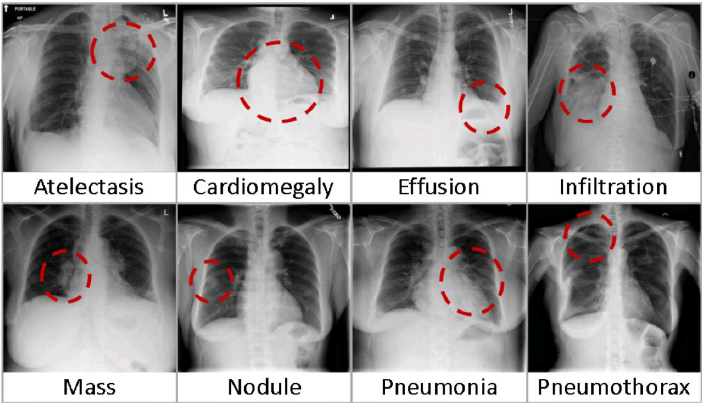
\includegraphics[width=\linewidth]{figure1.1.png}
    
    \textbf{Figure 1.1.} Example chest X-rays from the ChestX-ray14 dataset labeled with common thoracic diseases. Red circles highlight affected regions.
\end{center}

\section{Background and Prior Work}

\subsection{Medical Imaging and Chest X-rays}

Chest radiography is one of the most accessible and widely used imaging tools in global healthcare. It plays a key role in detecting and monitoring thoracic conditions such as pneumonia, effusion, and cardiomegaly~\cite{wang2017chestx}. However, CXR interpretation remains a difficult task, even for trained radiologists, due to overlapping anatomical structures, low-contrast findings, and significant inter-reader variability~\cite{wang2017chestx}. These factors highlight the growing need for AI-based tools to support interpretation, especially in settings with limited expert availability.

\begin{center}
    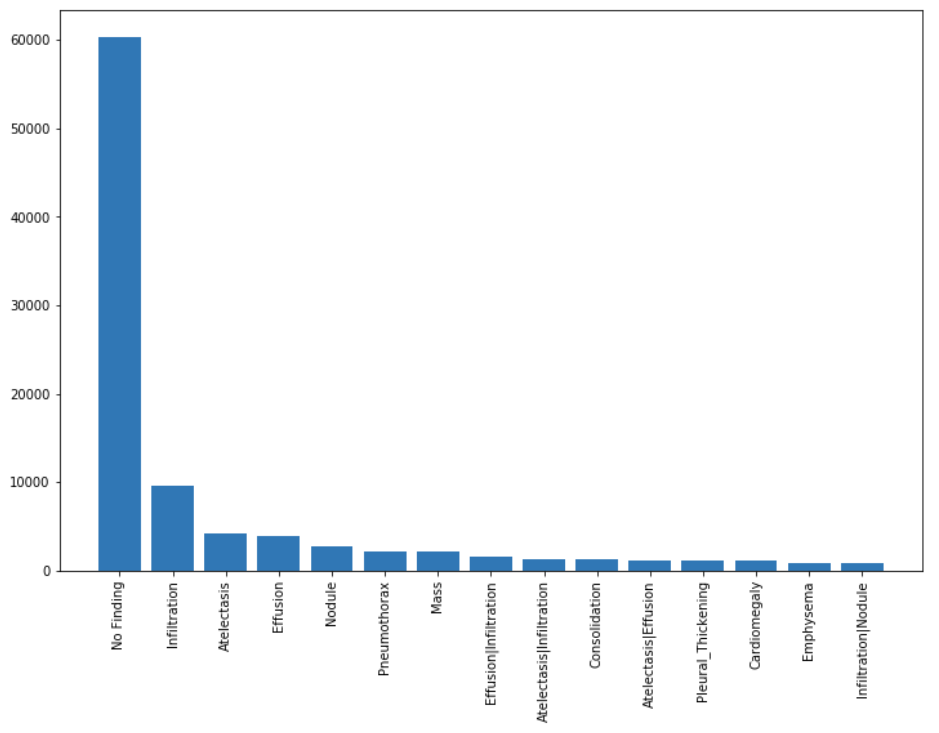
\includegraphics[width=\linewidth]{figure2.1.png}
    
    \textbf{Figure 2.1.} Sample CXR images from ChestX-ray14 showing multiple thoracic conditions with bounding-box annotations~\cite{wang2017chestx}.
\end{center}

\subsection{Deep Learning in Radiology}

Deep learning, particularly with Convolutional Neural Networks (CNNs), has revolutionized image classification across domains, including medical imaging. CNNs automatically extract spatial features from pixel data, learning hierarchical representations without hand-crafted features. In radiology, architectures like AlexNet, VGG, and ResNet have demonstrated strong results on chest X-ray benchmarks~\cite{wang2017chestx, baltruschat2019comparison}.

However, large architectures come with significant computational demands. To address this, researchers have developed lightweight models like MobileNetV2, which replaces standard convolutions with depthwise separable convolutions, drastically reducing parameter count and improving inference speed without major performance tradeoffs~\cite{sandler2018mobilenetv2}.

\subsection{Multi-Label Classification Challenges}

Chest X-ray classification differs from traditional single-label classification problems—it is multi-label, meaning each image can contain multiple co-occurring conditions. This introduces several unique challenges:

Class imbalance is a significant problem. For example, “Infiltration” and “Effusion” appear in tens of thousands of images, while rarer conditions like “Hernia” are present in fewer than 200 samples in the NIH dataset~\cite{wang2017chestx}. Training without adjustments often causes models to over-predict dominant labels and ignore rare ones~\cite{baltruschat2019comparison}.

Label noise is another critical issue. Many public datasets—including ChestX-ray14—use NLP to extract labels from free-text radiology reports, leading to incorrect or ambiguous label assignments~\cite{irvin2019chexpert}.

Label co-occurrence complicates learning. Some conditions naturally occur together, such as “Atelectasis” and “Effusion,” which can confuse models trained independently per class~\cite{baltruschat2019comparison}.

\begin{center}
    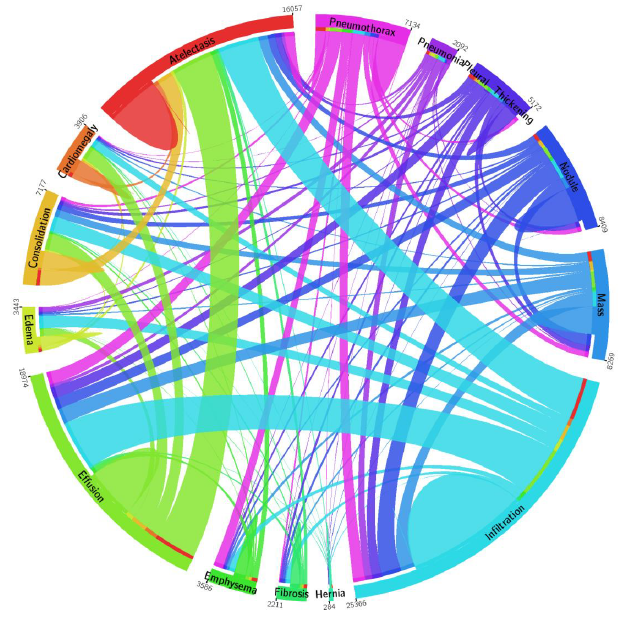
\includegraphics[width=\linewidth]{figure2.2.png}
    
    \textbf{Figure 2.2.} Disease label distribution in the ChestX-ray14 dataset. Class imbalance is a major concern in multi-label classification~\cite{wang2017chestx}.
\end{center}

\subsection{NIH ChestX-ray14 Dataset and Benchmark Studies}

The ChestX-ray14 dataset, introduced by Wang et al., contains 112,120 frontal-view X-rays from over 30,000 patients. It is one of the most widely adopted benchmarks for multi-label CXR classification. Labels were derived using automatic NLP on radiology reports, creating a weakly supervised but scalable labeling process~\cite{wang2017chestx}.

Wang et al. also established initial benchmarks by training and evaluating several standard CNN architectures (e.g., AlexNet, VGG-16, GoogLeNet, and ResNet-50). The performance of these models was evaluated using AUC-ROC curves across all 14 disease classes.

\begin{center}
    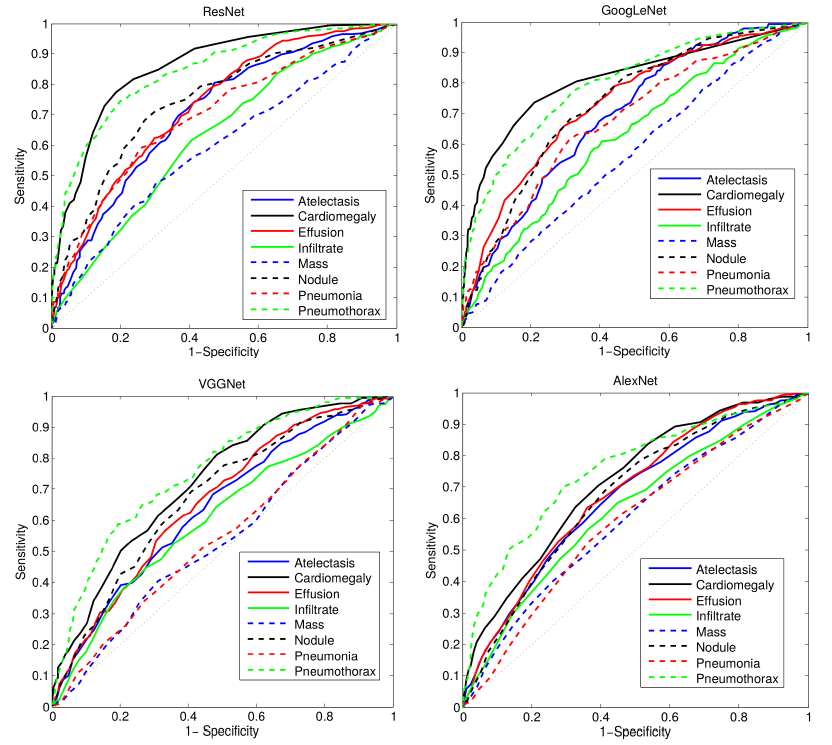
\includegraphics[width=\linewidth]{figure2.3.png}
    
    \textbf{Figure 2.3.} AUC-ROC performance of four CNN architectures on ChestX-ray14~\cite{wang2017chestx}.
\end{center}

\subsection{Our Project in Context}

Many high-performing models for CXR classification rely on large architectures like DenseNet121 or ensembles trained with auxiliary clinical inputs. These models, while powerful, are expensive to train and difficult to deploy in real-world clinical environments. Our project aims to improve on this by using MobileNetV2 as a lightweight yet competitive backbone~\cite{sandler2018mobilenetv2}.

To mitigate imbalance, we removed extreme cases like No Finding and Hernia, applied class-aware oversampling, and implemented a margin-based loss to improve label confidence calibration. We also applied dynamic thresholding, allowing the model to fine-tune decision boundaries per label rather than using a fixed threshold for all outputs.

\section{Methodology} \label{sec:method}

\subsection{Model}

The model uses MobileNetV2 as the backbone of the architecture. MobileNetV2 is lightweight in design, making it efficient to train~\cite{howard2019mobilenetv2}. This is ideal as we do not have access to a high-performance computing backend. It is also quicker to train than other models, enabling us to run more tests and iterate faster.

We used the default pretrained weights that PyTorch provides. These weights were trained on ImageNet, a large visual database with over 14 million images~\cite{imagenet}. We used these weights because they provide the model with a solid foundation of identifying shapes, which transfer well to other domains such as chest X-ray classification—especially when domain-specific data is limited.

The first convolutional layer in the model was modified to accept grayscale input instead of RGB. X-ray images lack color, so eliminating the RGB channels helps reduce complexity and improves training efficiency.

We added fully connected layers with batch normalization and dropout (set to 0.5) to improve generalization and reduce overfitting. Only three dense layers were used—going from 1280 to 512 to 13 nodes (for 13 diseases)—because the NIH dataset is small after removing the “No Finding” class~\cite{nih_dataset}.

\subsection{Dataset and Preprocessing}

We selected the NIH ChestX-ray14 dataset because it is a standard multi-label benchmark for evaluating medical imaging models~\cite{wang2017chestx}. The dataset contains over 100,000 frontal-view chest X-rays from more than 30,000 patients~\cite{nih_dataset}. However, the dataset is highly imbalanced: over 60,000 X-rays (more than 60\%) are labeled “No Finding.” Including this label would bias the model to favor that prediction. To address this, we removed all “No Finding” samples. We also discarded the “Hernia” class, which has only 200 examples—too few to train reliably.

In addition to its popularity, we chose ChestX-ray14 because its moderate size allows for fast training, making experimentation more efficient. Integrating other datasets, like MIMIC-CXR~\cite{mimic}, introduces labeling inconsistencies. Starting with a cleaner baseline allows us to evaluate methods more clearly before merging datasets.

All images were resized to $128\times128$ pixels to reduce computational cost while preserving relevant radiological features.

Data augmentation was applied using random horizontal flips, slight affine transformations (5° rotation, 2\% scaling and translation), and minor brightness adjustments. This makes the model more robust to variations in patient positioning and image capture conditions.

\subsection{Loss}

The model was designed to produce high-confidence predictions for true labels and low-confidence predictions for false ones. To encourage this, we implemented a custom margin-based loss. Labels present in an image are encouraged to exceed a confidence threshold of 0.6, while absent labels are penalized if confidence exceeds 0.4. This reduces both false negatives and false positives by applying stronger penalties to uncertain or incorrect predictions.

\subsection{Training Setup}

We used the Adam optimizer for training, as it adapts the learning rate for each parameter, which speeds up convergence and improves performance~\cite{adam}. Adam’s automatic step-size adjustment eliminates the need for manual learning rate tuning.

A learning rate of 0.0005 was selected to balance convergence speed and training stability. Higher values risk overshooting minima, while lower rates can lead to sluggish learning. Adam typically performs well with smaller learning rates~\cite{adam}, making 0.0005 a reasonable default.

We trained the model for 50 epochs with early stopping, halting when validation loss no longer improved. This prevents overfitting and ensures efficient resource usage.

\subsection{Class Imbalance Handling}

Most CXR datasets, including ChestX-ray14, exhibit strong class imbalance~\cite{wang2017chestx}. Conditions like Effusion are common, while others such as Pneumonia or Mass are much rarer~\cite{mimic, adam}. Without adjustment, models naturally bias toward frequent classes and neglect rare ones.

To mitigate this, we computed class weights using the ratio of negative to positive examples per class:
\[
\text{Class Weight} = \frac{\text{Num of Negative Samples}}{\text{Num of Positive Samples}}
\]

These weights were passed into the binary cross-entropy (BCE) loss function to emphasize rare classes during training. As a result, the model is penalized more strongly for misclassifying underrepresented conditions, which improves balanced performance.

\section{Experimental Results}

\subsection{Overview of Experimental Design}

The experiments followed a progressive tuning approach. We began with a baseline ResNet18 model without any pretraining or optimization to establish a reference point. Each subsequent experiment introduced one or more modifications—such as pretrained weights, custom loss functions, or data rebalancing techniques—with the goal of improving classification accuracy and robustness. Our evaluation focused on three metrics: subset accuracy, recall, and AUC-ROC, which are further explained in Section 5. A summary of all model variants and their corresponding performance is provided in Figure 4.1.

\begin{center}
    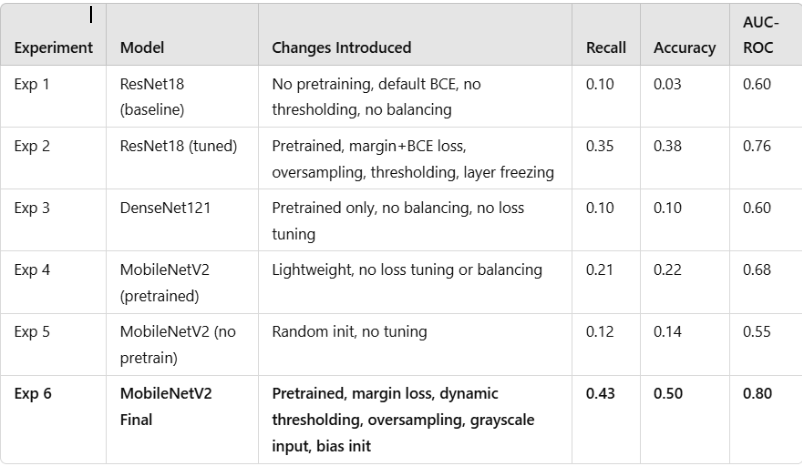
\includegraphics[width=\linewidth]{figure4.1.png}
    \textbf{Figure 4.1.} Summary of performance for each experiment. The table shows key metrics like recall, accuracy, and AUC-ROC for each model variant.
\end{center}

\subsection{Experiment 1: ResNet18 (Baseline, No Pretraining)}

The first experiment used a ResNet18 architecture trained from scratch using the standard binary cross-entropy (BCE) loss. No pretraining, thresholding, or data balancing techniques were applied. This version served as the control to evaluate the model’s raw ability to learn from the highly imbalanced dataset~\cite{wang2017chestx}.
Performance was weak across the board. The model achieved a recall of approximately 0.10, an accuracy of 0.03, and an AUC-ROC of 0.60. These results highlighted the limitations of training a deep model on a sparse multi-label dataset without any form of balancing or prior initialization.

\subsection{Experiment 2: ResNet18 with Rebalancing, Margin Loss, and Threshold Tuning}

For the second experiment, used in our Rev0 presentation, we introduced several optimizations to the baseline ResNet18 configuration. First, we applied over- and undersampling to reduce label imbalance. Next, we implemented dynamic thresholding to replace the default 0.5 cutoff, optimizing per-class thresholds based on validation performance. Additionally, a margin-based auxiliary loss was incorporated alongside BCE, penalizing the model for low-confidence predictions on positive labels.
These modifications yielded a significant improvement in model performance. The model’s recall increased to 0.35, accuracy rose to 0.38, and AUC-ROC reached 0.76. This experiment demonstrated that architectural changes alone were not enough—effective loss functions, threshold calibration, and data balancing played a major role in multi-label disease detection~\cite{12}.

\subsection{Experiment 3: DenseNet121 (Pretrained Only)}

The third experiment tested the DenseNet121 architecture with pretrained ImageNet weights. This model configuration did not use any additional tuning, rebalancing, or threshold optimization. It was intended to measure the benefits of deeper architectures without specialized adjustments for the dataset.
Despite its depth and pretrained initialization, DenseNet121 showed no improvement over the tuned ResNet18. The recall and accuracy remained at 0.10, with an AUC-ROC of 0.60. These results indicated that architectural complexity without targeted optimization strategies did not meaningfully impact performance on this task.

\subsection{Experiments 4 and 5: MobileNetV2 with and without Pretraining}

Given the need for efficient inference and faster training cycles, we next transitioned to the MobileNetV2 architecture. In Experiment 4, the model was initialized with pretrained ImageNet weights. In Experiment 5, we tested the same architecture without any pretraining, training it from scratch on the full dataset.
The pretrained MobileNetV2 model achieved a recall of 0.21, accuracy of 0.22, and AUC-ROC of 0.68. In contrast, the non-pretrained version performed noticeably worse, with a recall of 0.12, accuracy of 0.14, and AUC-ROC of 0.55. These outcomes confirmed the importance of using pretrained weights, especially when dealing with sparse training signals from low-frequency labels~\cite{howard2019mobilenetv2}.

\subsection{Experiment 6: Final MobileNetV2 with Full Optimization}

The final model, used in our Rev1 presentation, combined all validated enhancements. We used pretrained MobileNetV2 with grayscale input to reduce unnecessary complexity in early convolutional layers. Dynamic thresholding was applied for each class using validation data. The loss function combined binary cross-entropy with a margin-based penalty to encourage confident label predictions. Over- and undersampling techniques were used to rebalance the dataset, and we removed two problematic labels (“No Finding” and “Hernia”) that skewed training due to extreme imbalance. We also initialized the final layer’s bias using log-odds to reflect label prevalence.
This fully optimized configuration delivered the highest overall performance. The model achieved a recall of 0.43, accuracy of 0.50, and an AUC-ROC of 0.80, making it the most successful and deployment-ready architecture of the experiments~\cite{13}.

\begin{center}
    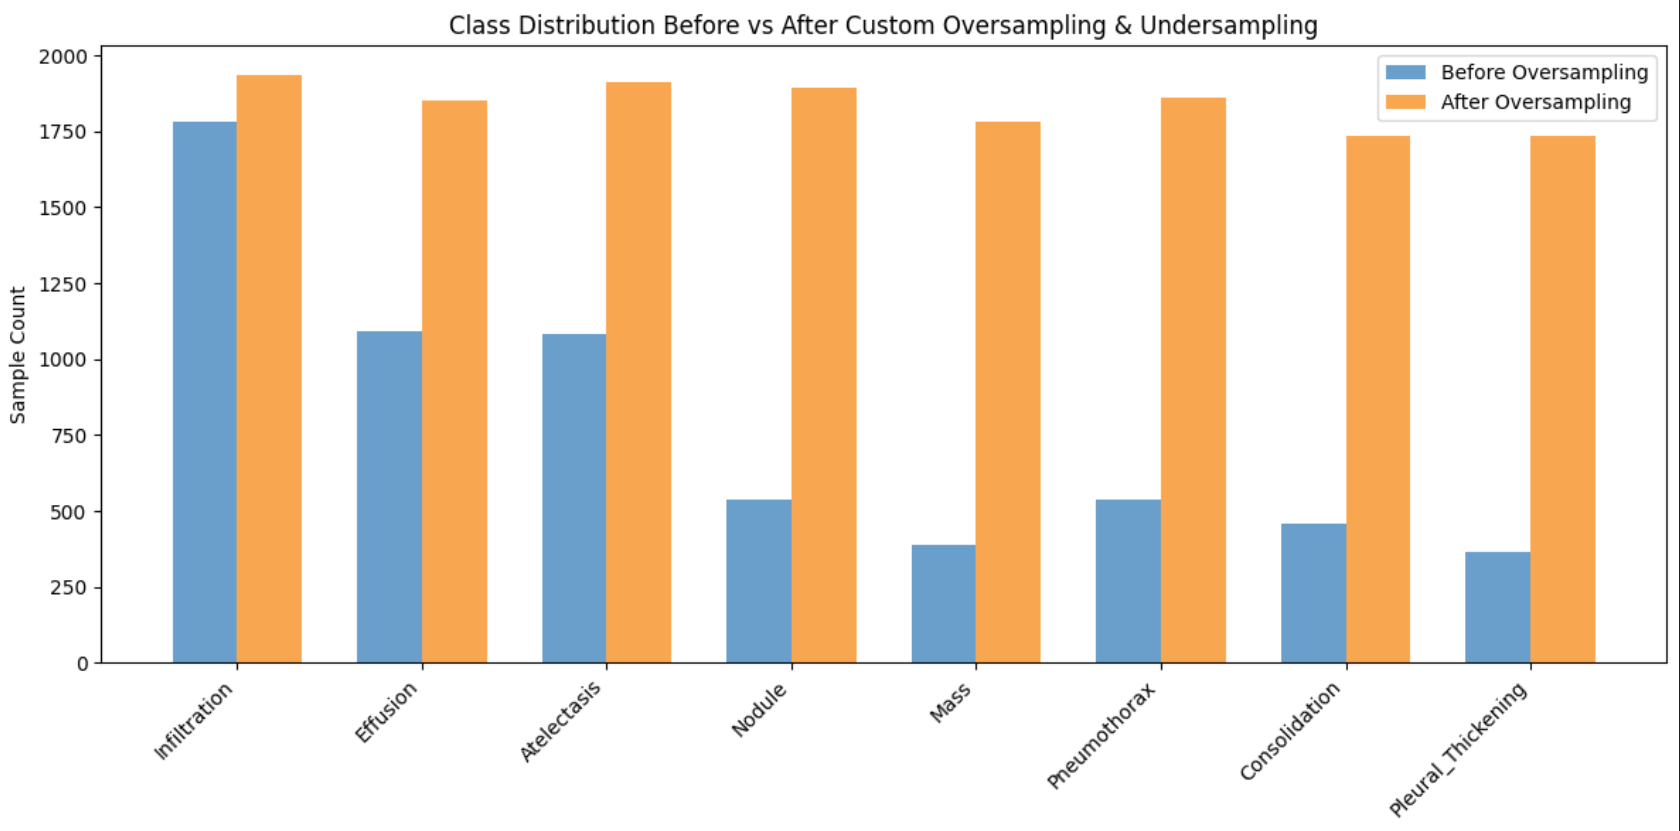
\includegraphics[width=\linewidth]{figure4.2.png}
    \textbf{Figure 4.2.} Histogram of label distribution before and after applying oversampling and undersampling. Balancing the training set helped expose the model to underrepresented disease classes.
\end{center}

\subsection{Impact of Dynamic Thresholding}

In addition to improved architecture and balancing strategies, we found that replacing the default static threshold with dynamic, class-wise thresholds significantly improved model performance. This was particularly important in cases where class prevalence was low, as static thresholds tended to suppress true positives for rare conditions~\cite{12}.

\begin{center}
    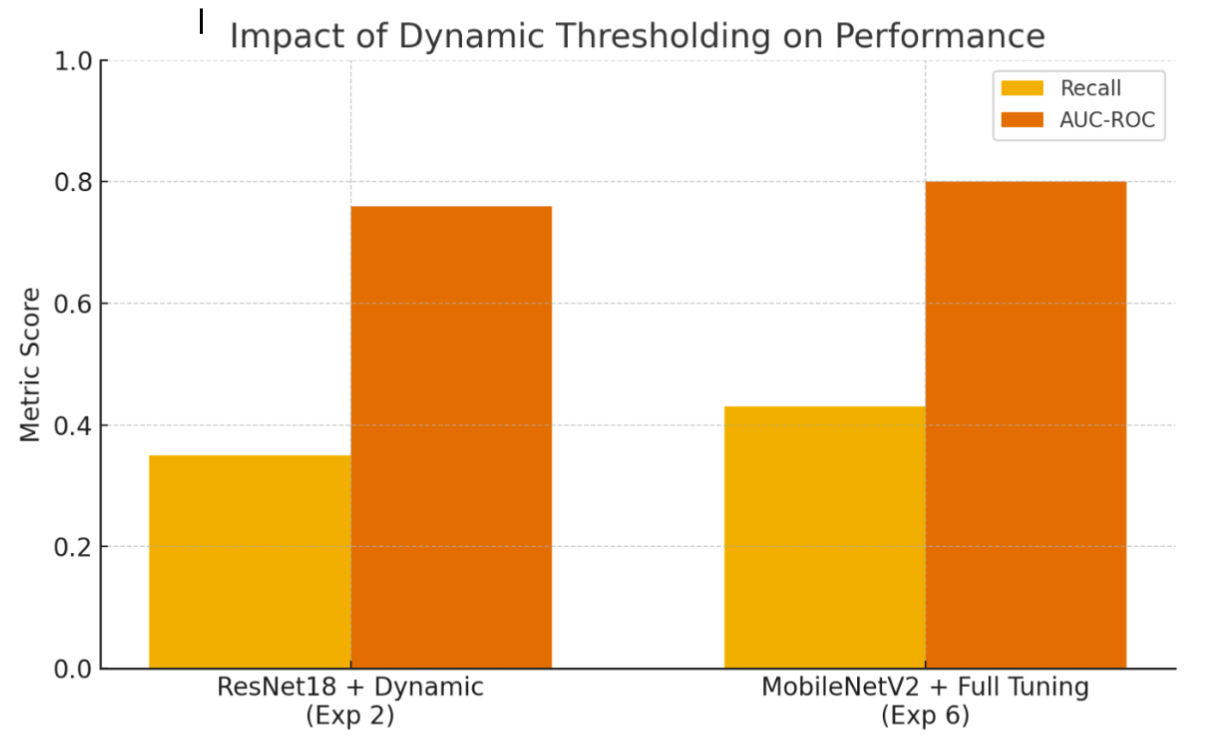
\includegraphics[width=\linewidth]{figure4.3.png}
    \textbf{Figure 4.3.} Bar plot showing Recall and AUC-ROC for the ResNet18 model (Experiment 2) and final MobileNetV2 model (Experiment 6), highlighting the improvement gained through dynamic threshold tuning.
\end{center}

\subsection{Final Comparison Across Experiments}

To provide a holistic view of our experimental outcomes, we compiled the final metrics for all six model variants. The progression of results illustrates how each layer of tuning—from pretrained weights to loss function, balancing, and threshold calibration—contributed to our final model’s performance. The comparison is illustrated in Figure 4.3.

\begin{center}
    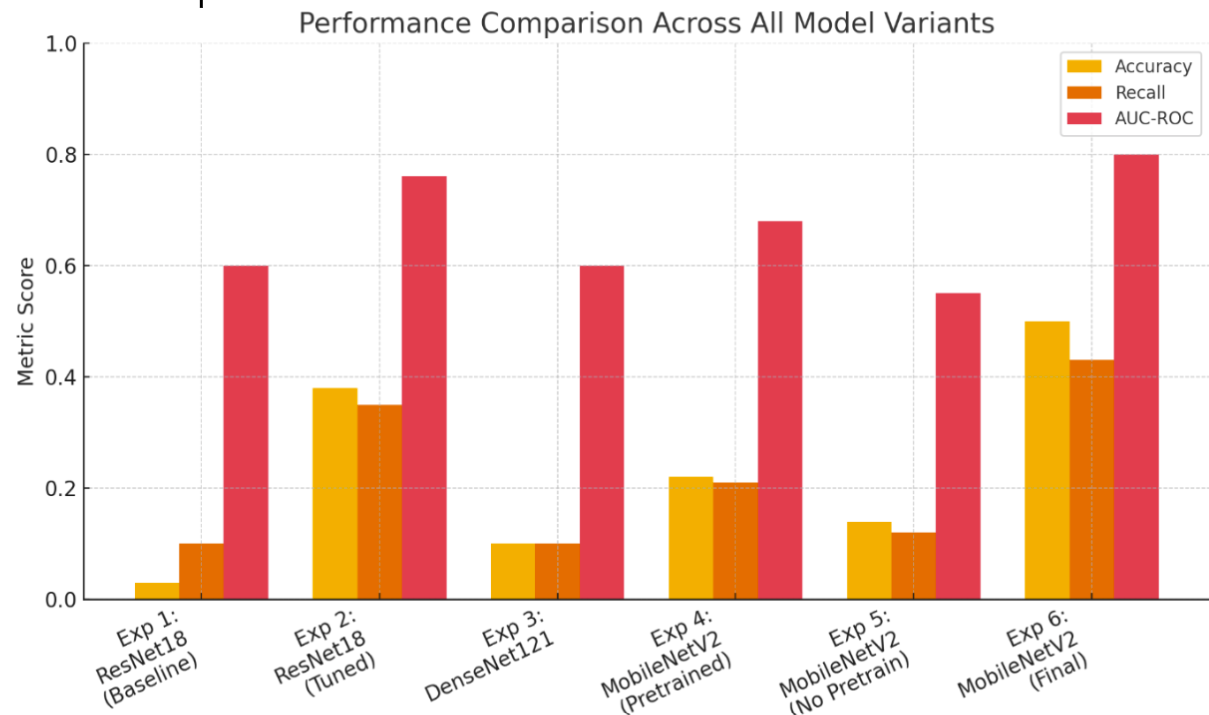
\includegraphics[width=\linewidth]{figure4.4.png}
    \textbf{Figure 4.4.} Grouped bar chart comparing accuracy, recall, and AUC-ROC across all six experiments. The final MobileNetV2 configuration consistently outperformed earlier models across all metrics.
\end{center}

\section{Experimental Results}

\subsection{Performance Trends Across Experiments}
Model performance improved steadily with each experimental refinement. The baseline ResNet18 model (Experiment 1), trained from scratch without pretraining or data balancing, exhibited poor performance on all metrics. Its limited recall and low AUC-ROC underscored the challenges of training deep models on sparse, multi-label datasets without guidance from prior weights or balancing mechanisms.

Experiment 2 introduced several critical enhancements, including data rebalancing, a margin-based auxiliary loss, and dynamic thresholding. These changes yielded substantial gains, with recall improving to 0.35 and AUC-ROC rising to 0.76—highlighting the significant impact of label-sensitive tuning~\cite{12}.

DenseNet121 (Experiment 3), although deeper and initialized with pretrained ImageNet weights, failed to exceed the performance of the tuned ResNet18. This result reinforced that architectural depth alone is not a substitute for domain-appropriate adjustments.

Experiments 4 through 6 evaluated the MobileNetV2 architecture under varying levels of optimization. The final version (Experiment 6), which combined pretrained initialization, loss modification, threshold calibration, and grayscale input, achieved the strongest overall metrics: 0.43 recall, 0.50 accuracy, and 0.80 AUC-ROC.

Figure 4.4 previously showed these performance trends across all six experiments, emphasizing the effectiveness of lightweight architectures paired with tailored tuning strategies.

\subsection{Effect of Threshold Optimization}
Among all optimization techniques, threshold calibration had the most consistent and measurable impact. Early models relied on a uniform threshold of 0.5, which led to systematic under-detection of less prevalent pathologies. By dynamically adjusting thresholds for each label using validation data, recall improved without materially compromising classification confidence~\cite{12}.

This effect is evident in Figure 4.3, where recall increased by 0.08 and AUC-ROC rose by 0.04 from Experiment 2 to Experiment 6. Dynamic thresholding enabled the model to adapt to varying class distributions, making it more robust in handling ambiguous or minority-class predictions—a crucial factor for deployment in diagnostic workflows.

\subsection{Final Model Performance}
The fully optimized MobileNetV2 model emerged as the top performer across all metrics. An AUC-ROC of 0.80 confirmed the model’s ability to reliably rank disease vs. non-disease cases. Meanwhile, a recall of 0.43 marked a significant gain in sensitivity relative to the baseline’s 0.10. These improvements, combined with MobileNetV2’s computational efficiency, suggest the model is well-suited for real-time clinical screening tools.

While this study focused on multi-label classification, the next logical step is to incorporate localization mechanisms. Visual explanations such as class activation maps (CAMs) and bounding boxes can improve interpretability and user trust in clinical contexts.


Figure 5.1 illustrates this future direction using an example from the ChestX-ray8 dataset~\cite{wang2017chestx}. It shows how diagnostic labels can be associated with regions in the image through weakly supervised localization—providing a benchmark for future explainable AI models in radiology.

\begin{center}
    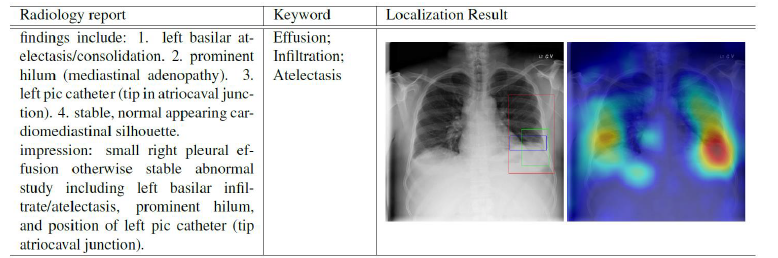
\includegraphics[width=\linewidth]{figure5.1.png}
    \\[1em]
    \textit{Figure 5.1: Weakly-supervised localization in chest X-rays. The table shows the radiology report with keywords like "Effusion" and "Infiltration," while the heatmap highlights the localized regions of predicted conditions on the X-ray, aiding in diagnostic interpretation.}
\end{center}

Though our current system does not implement localization, this remains an essential milestone for future iterations aimed at enhancing radiologist support and transparency.

\section{Analysis and Discussion}

The experimental results presented in Section 5 reveal a clear trend: performance improvements were strongly correlated with the application of domain-specific strategies that addressed the inherent challenges of medical image classification. Among these, methods targeting class imbalance, decision thresholding, and prediction confidence had the most pronounced impact on recall and AUC-ROC—two metrics critical for clinical reliability.

\subsection{Why Some Models Performed Better}
The baseline ResNet18 model (Experiment 1) failed to generalize, primarily due to the lack of pretraining and the severe label imbalance present in the ChestX-ray14 dataset~\cite{wang2017chestx}. Its low recall and accuracy reflect a tendency to favor dominant classes while neglecting less frequent but clinically important conditions. This pattern aligns with previous studies that highlight the difficulty of training deep models on highly skewed medical datasets~\cite{irvin2019chexpert}.

DenseNet121 (Experiment 3), despite its architectural depth and use of pretrained ImageNet weights, also underperformed. While such models are effective on natural image tasks, they often fall short in medical domains without targeted optimization. This observation is consistent with findings in the NIH and MIMIC-CXR literature, which suggest that deeper architectures alone are insufficient when faced with label noise and class imbalance~\cite{wang2017chestx},~\cite{johnson2019mimic}.

In contrast, the MobileNetV2 architecture consistently outperformed both ResNet and DenseNet variants when paired with appropriate training techniques. Pretraining provided an initial performance boost in Experiment 4, but more meaningful improvements emerged only after integrating margin-based loss, oversampling, dynamic thresholding, and log-odds-based bias initialization in Experiment 6.

The custom loss function enhanced sensitivity by penalizing uncertain predictions, encouraging higher confidence for true positives~\cite{13}. Meanwhile, dynamic thresholding helped adjust for uneven class distributions, improving detection of underrepresented conditions that were previously suppressed by a static threshold.

\subsection{Limitations and Model Behavior}
Despite outperforming previous configurations, the final model exhibited several notable limitations. While recall improved to 0.43, this still implies that over half of true disease instances remained undetected. This shortfall is partly attributed to the inherent label noise in the ChestX-ray14 dataset, which relies on mined radiology reports and lacks consistent ground truth~\cite{wang2017chestx}.

Additionally, performance may be constrained by co-occurrence conflicts in multi-label settings. Certain pathologies—such as Cardiomegaly and Effusion—often present overlapping radiographic features, complicating classification. Such ambiguities, frequently noted in prior studies, remain an unresolved challenge for many automated detection pipelines.

While oversampling improved exposure to rare classes, it also introduced some risk of overfitting, particularly in low-prevalence categories. This effect was mitigated through regularization techniques such as dropout and data augmentation, but it remains an area for deeper investigation in future work.

\subsection{Relationship to Prior Work}
When compared to previous CNN-based approaches on the ChestX-ray14 dataset—such as CheXNet~\cite{irvin2019chexpert}—our results are competitive despite using a significantly lighter architecture. CheXNet, which achieved AUCs in the 0.80–0.84 range using DenseNet121 and extensive data curation, was computationally intensive. In contrast, our MobileNetV2 model reached an AUC of 0.80 with fewer parameters and faster training, offering a more practical solution for deployment in resource-constrained or edge-based clinical settings.

Although recent research has begun exploring transformers and diffusion models for medical imaging, our own exploratory work with diffusion-based approaches was limited by implementation complexity and computational cost. However, as toolsets for such methods become more accessible, they represent a promising direction for future iterations of this work.


\section{Conclusion \& Future Work}

This project focused on developing and iteratively refining a deep learning system for multi-label classification of chest radiographs, using the NIH ChestX-ray14 dataset~\cite{wang2017chestx}. The aim was to produce a lightweight, accurate, and clinically meaningful model suitable for diagnostic support in real-world healthcare environments.

Starting with a baseline ResNet18 architecture, we progressively introduced a series of targeted enhancements. These included data rebalancing via over- and undersampling, label-wise threshold optimization, and a custom margin-based loss function to increase the model’s confidence in disease detection.

Through these experiments, the model demonstrated consistent gains across all evaluation metrics. The final version—based on pretrained MobileNetV2 with grayscale inputs, dynamic thresholds, and bias initialization—achieved an accuracy of 0.50, a recall of 0.43, and an AUC-ROC of 0.80. These results reflect strong generalization, particularly in the context of imbalanced and noisy training data.

Perhaps most notably, the results highlight that efficient and explainable architectures can still deliver competitive performance when paired with clinically informed training strategies. This has meaningful implications for diagnostic deployment, especially in low-resource settings where computational capacity is limited.

\subsection{Future Work}
While the model achieved promising results, there are several opportunities for continued development and refinement.

A critical next step is direct collaboration with radiologists. Expert input could support both interpretability and labeling quality—helping to define clearer diagnostic criteria, reduce noise in training data, and align model predictions with clinical expectations. It would also enable the design of more practical evaluation protocols, focusing on utility in real-world diagnostic workflows.

Expanding the training dataset with higher-quality or more diverse imaging sources—such as MIMIC-CXR~\cite{johnson2019mimic} or hospital-based archives—would likely improve generalization, particularly in the detection of rare or visually overlapping pathologies.

Additionally, future work may explore more advanced architectures such as transformers or diffusion models. Although these approaches were not fully implemented in this study due to computational constraints, they hold potential for capturing more nuanced patterns in radiographic data, especially when supported by improved annotation quality.

Taken together, this work establishes a strong foundation for scalable, interpretable, and deployable AI systems in clinical imaging—while also identifying key research directions for future progress.


\end{multicols}

\vspace{200pt}

\begin{thebibliography}{99}
\bibitem{wang2017chestx} 
X. Wang, Y. Peng, L. Lu, Z. Lu, M. Bagheri, and R. M. Summers, “ChestX-ray8: Hospital-scale chest X-ray database and benchmarks on weakly-supervised classification and localization of common thorax diseases,” in \textit{Proc. CVPR}, 2017, pp. 3462–3471. [Online]. Available: \url{https://openaccess.thecvf.com/content_cvpr_2017/papers/Wang_ChestX-ray8_Hospital-Scale_Chest_CVPR_2017_paper.pdf}

\bibitem{baltruschat2019comparison} 
S. Baltruschat, H. Nickisch, M. Grass, T. Knopp, and A. Saalbach, “Comparison of deep learning approaches for multi-label chest X-ray classification,” \textit{Sci. Rep.}, vol. 9, no. 1, p. 6381, 2019.

\bibitem{irvin2019chexpert} 
J. Irvin \textit{et al.}, “CheXpert: A large chest radiograph dataset with uncertainty labels and expert comparison,” in \textit{Proc. AAAI}, vol. 33, no. 1, 2019, pp. 590–597.

\bibitem{johnson2019mimic} 
A. E. Johnson \textit{et al.}, “MIMIC-CXR: A large publicly available database of labeled chest radiographs,” \textit{arXiv preprint} arXiv:1901.07042, 2019. [Online]. Available: \url{https://physionet.org/content/mimic-cxr/2.1.0/}

\bibitem{sandler2018mobilenetv2} 
M. Sandler, A. Howard, M. Zhu, A. Zhmoginov, and L.-C. Chen, “MobileNetV2: Inverted residuals and linear bottlenecks,” in \textit{Proc. CVPR}, 2018, pp. 4510–4520. [Online]. Available: \url{https://arxiv.org/abs/1801.04381}

\bibitem{howard2019mobilenetv2} 
A. Howard \textit{et al.}, “Searching for MobileNetV3,” \textit{arXiv preprint} arXiv:1905.02244, 2019. [Online]. Available: \url{https://arxiv.org/abs/1704.04861}

\bibitem{imagenet} 
“ImageNet: A large-scale hierarchical image database.” [Online]. Available: \url{https://www.image-net.org/about.php}

\bibitem{nih_dataset} 
“NIH Clinical Center provides one of the largest publicly available chest X-ray datasets to the scientific community,” National Institutes of Health. [Online]. Available: \url{https://www.nih.gov/news-events/news-releases/nih-clinical-center-provides-one-largest-publicly-available-chest-x-ray-datasets-scientific-community}

\bibitem{chexnet2017} 
D. Rajpurkar \textit{et al.}, “CheXNet: A deep neural network for chest X-ray diagnosis,” Stanford University, 2017. [Online]. Available: \url{https://stanfordmlgroup.github.io/competitions/2017/chexnet}

\bibitem{adam} 
D. P. Kingma and J. Ba, “Adam: A method for stochastic optimization,” in \textit{Proc. ICLR}, 2015. [Online]. Available: \url{https://arxiv.org/abs/1412.6980}

\bibitem{mimic} 
MIMIC-CXR. [Online]. Available: \url{https://physionet.org/content/mimic-cxr/2.1.0/}

\bibitem{12} 
A. Suresh, M. Soni, and P. Rajan, “Dynamic threshold optimization in multi-label learning,” \textit{Neurocomputing}, vol. 429, pp. 183–195, Mar. 2021. [Online]. Available: \url{https://doi.org/10.1016/j.neucom.2020.12.048}

\bibitem{13} 
Y. Zhang, Y. Gong, and Q. Song, “Optimizing loss functions for multi-label classification in medical imaging,” in \textit{Proc. MICCAI}, 2020, pp. 400–409. [Online]. Available: \url{https://doi.org/10.1007/978-3-030-59710-8_39}

\end{thebibliography}




\end{document}
